% =====================================================================
%  Plan4ARI -- D4.1 (A4 revision) -- Supporting note
%  State of the art on Model Predictive Path Integral (MPPI) control
%  for industrial manipulators and Autonomous Mobile Robots (AMRs)
%
%  Build:  latexmk -pdf main.tex      (or: pdflatex, bibtex, pdflatex x2)
%  Sources: ../wiki/sources/<bibkey>.md   PDFs: ../raw/papers/<bibkey>.pdf
% =====================================================================
\documentclass[10pt,a4paper]{article}

\usepackage[utf8]{inputenc}
\usepackage[T1]{fontenc}
\usepackage{lmodern}
\usepackage[a4paper,margin=2.1cm]{geometry}
\usepackage{amsmath,amssymb,bm}
\usepackage{booktabs,tabularx,multirow}
\usepackage{graphicx}
\usepackage[dvipsnames]{xcolor}
\usepackage{tikz}
\usetikzlibrary{arrows.meta,positioning,fit,backgrounds}
\usepackage{algorithm}
\usepackage{algpseudocode}
\usepackage{enumitem}
\usepackage{cite}
\usepackage{microtype}
\usepackage[colorlinks=true,linkcolor=MidnightBlue,citecolor=MidnightBlue,urlcolor=MidnightBlue]{hyperref}

\setlist{itemsep=1pt,topsep=3pt,leftmargin=*}
% Macros used by sota_body.tex
\providecommand{\E}{\mathbb{E}}
\providecommand{\KL}{\mathbb{D}_{\mathrm{KL}}}
\providecommand{\U}{\bm{U}}
\providecommand{\V}{\bm{V}}
% \sotafullfalse (set by the D4.1 before % sota_body.tex -- body of the MPPI state-of-the-art note.
% Included by main.tex (standalone SOTA note) and by the D4.1 deliverable (D4.1-latex).
% Requires: amsmath, bm, algorithm, algpseudocode, tikz (arrows.meta, positioning), tabularx, booktabs, sota_macros.tex.
% ---------------------------------------------------------------------
\ifsotafull
\section{Scope and motivation}
% ---------------------------------------------------------------------
Plan4ARI targets teams of mobile manipulators and industrial arms working in dynamic, human-shared environments. Its baseline architecture couples informed sampling-based planning (global, \emph{Open IPC}) with MPC-based reference generation and micro-interpolation (local, \emph{Core IPC}). Two requirements stress this baseline: (i) \emph{reactivity}, i.e.\ replanning within tens of milliseconds when humans, AGVs or objects move, and (ii) \emph{expressiveness of the objective}: non-smooth costs (collision, separation distance, task switching, contact) that are awkward for gradient-based solvers. MPPI addresses both: it optimises an arbitrary cost by forward-simulating thousands of perturbed control sequences in parallel and averaging them with information-theoretic weights~\cite{williams2017jgcd,williams2018tro}. The review below was built from 69 sources (52 retrieved as full text and organised in an LLM-maintained wiki, see \texttt{../wiki/index.md}); recent surveys~\cite{kazim2024survey} were used to cross-check coverage.

\fi
% ---------------------------------------------------------------------
\section{Theoretical framework}
% ---------------------------------------------------------------------
\paragraph{Path integral control.}
Consider control-affine stochastic dynamics $d\bm{x} = \bm{f}(\bm{x})dt + \bm{G}(\bm{x})(\bm{u}\,dt + d\bm{w})$, $\E[d\bm{w}\,d\bm{w}^\top]=\bm{\Sigma}\,dt$, and the cost $J=\E\big[\phi(\bm{x}_T)+\int_0^T q(\bm{x}_t)+\tfrac12\bm{u}_t^\top\bm{R}\bm{u}_t\,dt\big]$. The value function obeys a nonlinear Hamilton--Jacobi--Bellman (HJB) PDE. Kappen~\cite{kappen2005pathintegrals} showed that, under the assumption $\lambda\bm{R}^{-1}=\bm{\Sigma}$ (noise is large where control is cheap), the exponential transformation $V=-\lambda\log\Psi$ makes the HJB \emph{linear} in the desirability $\Psi$. Through the Feynman--Kac lemma the solution becomes an expectation over uncontrolled trajectories,
\begin{equation}
\Psi(\bm{x}_0,0)=\E_{p}\!\left[\exp\!\big(-\tfrac{1}{\lambda}S(\tau)\big)\right],\qquad
\bm{u}^*(t)\,dt=\frac{\E_{p}\!\left[\exp(-S(\tau)/\lambda)\,d\bm{w}_t\right]}{\E_{p}\!\left[\exp(-S(\tau)/\lambda)\right]},
\label{eq:pi}
\end{equation}
where $S(\tau)=\phi(\bm{x}_T)+\int q\,dt$ is the state cost of trajectory $\tau$. The optimal control is thus a \emph{cost-weighted average of noise}, computable by Monte-Carlo sampling without differentiating dynamics or cost. Theodorou \emph{et al.}~\cite{theodorou2010pi2} exploited this result for policy improvement (PI$^2$), and STOMP~\cite{kalakrishnan2011stomp} for offline trajectory optimisation.

\paragraph{Information-theoretic MPPI.}
Williams \emph{et al.} turned \eqref{eq:pi} into a receding-horizon controller~\cite{williams2016aggressive,williams2017jgcd} and later re-derived it in discrete time from an information-theoretic argument that removes the control-affine assumption~\cite{williams2017itmpc,williams2018tro}. Let $\V=(\bm{v}_0,\dots,\bm{v}_{T-1})$ be an input sequence sampled as $\bm{v}_t=\bm{u}_t+\bm{\epsilon}_t$, $\bm{\epsilon}_t\sim\mathcal{N}(\bm 0,\bm\Sigma)$, with density $q_{\U}$, and let $p$ be a base (prior) distribution. The free energy satisfies
\begin{equation}
-\lambda\log\E_{p}\!\left[e^{-S(\V)/\lambda}\right]\;\le\;\E_{q}[S(\V)]+\lambda\,\KL(q\,\|\,p),
\end{equation}
with equality for the optimal distribution $q^*(\V)=\eta^{-1}\exp(-S(\V)/\lambda)\,p(\V)$. MPPI chooses the Gaussian mean $\U$ that minimises $\KL(q^*\|q_{\U})$, which yields a closed-form importance-sampling estimate from $K$ rollouts:
\begin{equation}
\bm{u}_t\leftarrow\bm{u}_t+\sum_{k=1}^{K}w_k\,\bm{\epsilon}^k_t,\qquad
w_k=\frac{1}{\eta}\exp\!\Big(-\frac{1}{\lambda}\big(\tilde S_k-\rho\big)\Big),\qquad
\tilde S_k=S(\V_k)+\gamma\sum_{t}\bm{u}_t^\top\bm\Sigma^{-1}\bm{v}^k_t,
\label{eq:mppi}
\end{equation}
where $\rho=\min_k\tilde S_k$ ensures numerical stability, $\eta$ normalises the weights, and the second term of $\tilde S_k$ is the likelihood-ratio (control) cost arising from the change of measure ($\gamma=\lambda(1-\alpha)$ in~\cite{williams2018tro}). The \emph{inverse temperature} $1/\lambda$ interpolates between a plain average ($\lambda\to\infty$) and greedy selection of the best rollout ($\lambda\to0$). Algorithm~\ref{alg:mppi} summarises one control cycle; the warm-started, shifted mean makes MPPI an anytime, real-time-iteration scheme.

\begin{algorithm}[t]
\caption{One cycle of MPPI (receding horizon)}\label{alg:mppi}
\begin{algorithmic}[1]
\small
\Require state $\bm{x}_0$, nominal sequence $\U$, covariance $\bm\Sigma$, temperature $\lambda$, samples $K$, horizon $T$
\For{$k=1\dots K$ \textbf{in parallel}}
  \State sample $\bm{\epsilon}^k_{0:T-1}\sim\mathcal{N}(\bm 0,\bm\Sigma)$; \quad roll out $\bm{x}^k_{t+1}=\bm{F}(\bm{x}^k_t,\bm{u}_t+\bm{\epsilon}^k_t)$ \Comment{model or physics simulator}
  \State $\tilde S_k\gets \phi(\bm{x}^k_T)+\sum_t q(\bm{x}^k_t)+\gamma\,\bm{u}_t^\top\bm\Sigma^{-1}(\bm{u}_t+\bm{\epsilon}^k_t)$
\EndFor
\State $\rho\gets\min_k\tilde S_k$;\quad $w_k\gets\exp(-(\tilde S_k-\rho)/\lambda)/\eta$ \Comment{importance weights}
\State $\bm{u}_t\gets\bm{u}_t+\sum_k w_k\bm{\epsilon}^k_t$; optionally smooth $\U$ \Comment{e.g.\ Savitzky--Golay, splines}
\State apply $\bm{u}_0$; shift $\U$ by one step and re-initialise $\bm{u}_{T-1}$ \Comment{warm start}
\end{algorithmic}
\end{algorithm}

\paragraph{Properties and limitations.}
MPPI (i) needs neither gradients nor convexity, so collision indicators, costmaps, logical task predicates and contacts enter the cost directly; (ii) is embarrassingly parallel (GPU, and recently FPGA~\cite{desai2026fpgampi}); (iii) can use a black-box physics engine as model~\cite{pezzato2025isaacmppi,howell2022predictivesampling}. Its known weaknesses are equally relevant for industrial use: constraints are only soft (penalties), so feasibility is not certified; sample complexity grows with input dimension and horizon; the Gaussian proposal is unimodal and the weighted \emph{average} of rollouts belonging to different homotopy classes can be infeasible (``averaging-induced failure''~\cite{liu2026clusteringmppi}); injected noise produces chattering inputs~\cite{kim2022smppi}; and stability or recursive-feasibility guarantees of classical MPC~\cite{mayne2014mpc} do not carry over. Most of the literature reviewed in Sect.~\ref{sec:lit} addresses one of these points.

% ---------------------------------------------------------------------
\section{MPPI versus MPC and other horizon-based planners}\label{sec:cmp}
% ---------------------------------------------------------------------
Gradient-based nonlinear MPC (NMPC) solves at each step a deterministic nonlinear program, typically with SQP or interior-point methods and real-time iterations (e.g.\ \texttt{acados}~\cite{verschueren2022acados}); it handles hard state/input constraints, provides local optimality and, with terminal ingredients, stability and recursive feasibility~\cite{rawlings2017mpc,mayne2014mpc}. It is the natural tool for jerk/torque-limited reference generation, as in predictive inverse kinematics and trajectory scaling for industrial manipulators~\cite{faroni2019pik,faroni2020scaling}. Its weaknesses are the need for smooth models and costs, sensitivity to initialisation in non-convex scenes (it converges to the local minimum of the current homotopy class), and the difficulty of encoding contacts and discrete decisions. Differential dynamic programming/iLQR~\cite{tassa2012ilqg} shares these traits but adds time-varying feedback gains.

Sampling-based MPC replaces the NLP with a stochastic search. The Cross-Entropy Method~\cite{rubinstein1999cem,pinneri2020icem} refits a Gaussian on an elite subset, predictive sampling~\cite{howell2022predictivesampling} keeps the best sample, and MPPI uses soft Boltzmann weights; Wagener \emph{et al.}~\cite{wagener2019dmd} unified these schemes as instances of online (mirror-descent) learning, and Stein-variational MPC~\cite{lambert2020svmpc} generalises them to non-parametric, multimodal posteriors. Classical motion-planning trajectory optimisers (CHOMP, STOMP, TrajOpt~\cite{zucker2013chomp,kalakrishnan2011stomp,schulman2014trajopt}) solve similar problems offline over full paths, while mobile-robot local planners such as DWA~\cite{fox1997dwa} (one-step constant-velocity sampling) and TEB~\cite{rosmann2017teb} (sparse NLP over multiple topologies) are the industrial incumbents MPPI is replacing in Nav2~\cite{macenski2023nav2survey}. Table~\ref{tab:cmp} summarises the comparison.

\begin{table}[t]
\centering\small
\caption{Qualitative comparison of horizon-based planning/control methods relevant to Plan4ARI.}\label{tab:cmp}
\setlength{\tabcolsep}{4pt}
\begin{tabularx}{\textwidth}{@{}>{\raggedright}p{2.3cm}>{\raggedright}X>{\raggedright}X>{\raggedright}X>{\raggedright}X>{\raggedright\arraybackslash}X@{}}
\toprule
 & \textbf{NMPC (SQP/IPM)} & \textbf{iLQR / DDP} & \textbf{CEM / predictive sampling} & \textbf{MPPI and variants} & \textbf{DWA / TEB} \\
\midrule
Optimisation principle & Deterministic NLP, Newton-type & Riccati backward pass & Elite refit / best sample & Path-integral importance sampling & Velocity sampling / sparse NLP \\
Gradients of model \& cost & Required (2nd order) & Required & Not required & Not required & DWA: no; TEB: yes \\
Hard constraints & Yes (exact) & Via augmented Lagrangian & Penalties / rejection & Penalties; CBF, projection or termination in variants & Partially \\
Non-smooth cost, contacts, logic & Poor & Poor & Good & Good (simulator in the loop) & Limited \\
Multimodality & Single local optimum & Single local optimum & Unimodal Gaussian & Unimodal; multimodal in SVMPC, SVG-, M3P2I, CE-MPPI & TEB: parallel topologies \\
Theory & Stability, recursive feasibility & Local convergence & Weak & Free-energy optimality; tube/robust bounds~\cite{gandhi2021rmppi} & Heuristic \\
Typical rate (arm / AMR) & 100--1000\,Hz (small models) & 100--1000\,Hz & 20--200\,Hz on GPU & 20--170\,Hz on GPU & 10--50\,Hz \\
Industrial maturity & High (\texttt{acados}, PLC-grade) & Medium & Research & ROS\,2 Nav2, STORM, MPPI-Generic & High (ROS) \\
\bottomrule
\end{tabularx}
\end{table}

The emerging consensus is that the two families are complementary rather than competing: MPPI explores globally within the horizon and copes with non-smooth objectives, gradient-based MPC refines and certifies. Hybrid schemes already appear at both levels: cuRobo~\cite{sundaralingam2023curobo} seeds GPU L-BFGS with a particle-based (MPPI-like) optimiser and plans collision-free arm motions in about 30--50\,ms, while Aoyama \emph{et al.}~\cite{aoyama2026hybrid} alternate DDP steps with Hessian-shaped sampling to escape local minima.

% ---------------------------------------------------------------------
\section{Analysis of the literature}\label{sec:lit}
% ---------------------------------------------------------------------
\subsection{Algorithmic advances}
\paragraph{Robustness to disturbances and model error.} Tube-MPPI~\cite{williams2018tubemppi} pairs MPPI with an iLQG ancillary tracker; RMPPI~\cite{gandhi2021rmppi} adds an augmented nominal state and provides bounds on the free-energy growth, i.e.\ the first performance guarantee for MPPI. Ensemble MPPI~\cite{abraham2020emppi} samples model parameters and adapts them online; U-MPPI~\cite{mohamed2025umppi} propagates means and covariances with the unscented transform and adds risk-sensitive costs; covariance steering~\cite{yin2022covsteering} shapes the sampled trajectory distribution.

\paragraph{Constraints and safety.} This is the most active line and the most relevant for certification. Shield-MPPI~\cite{yin2023shieldmppi} and SC-MPPI~\cite{gandhi2023safeis} embed control barrier functions (CBFs) in the cost or directly in forward sampling; GS-MPPI~\cite{rabiee2025gsmppi} uses composite CBFs so that \emph{all} sampled trajectories are safe; BR-MPPI~\cite{parwana2025brmppi} treats barrier rates as additional inputs and projects samples on the constraint manifold; BSS-MPPI~\cite{yin2024ccmppi} enforces chance constraints in belief space. For manipulators, PR-MPPI~\cite{lee2026prmppi} projects sampled joint velocities on equality (closed-chain) and inequality (joint-limit, clearance) constraints and retracts the result, achieving exact constraint satisfaction on 14-DoF dual-arm systems, while COSMIK-MPPI~\cite{gursoy2026cosmik} enforces human--robot separation by treating violations as rollout terminations (\emph{constraints-as-terminations}) and reports 100\% success at a constant 22\,ms per cycle, where gradient-based MPC failed in cluttered scenes.

\paragraph{Sampling distribution, smoothness and multimodality.} Smooth-MPPI~\cite{kim2022smppi} samples in the derivative-action space to remove chattering without post-filtering; log-MPPI~\cite{mohamed2022logmppi} uses normal--log-normal noise for better exploration of costmaps; Biased-MPPI~\cite{trevisan2024biasedmppi} re-derives MPPI for arbitrary proposal distributions and mixes samples from ancillary controllers (e.g.\ a global planner, a learned policy, a braking controller), alleviating local minima. MPOPI~\cite{asmar2023mpopi} adapts the proposal through adaptive importance sampling, and Tsallis-divergence VI-MPC~\cite{wang2021tsallis} generalises the exponential weighting. Multimodality is handled by Stein variational methods (SVMPC~\cite{lambert2020svmpc}, SVG-MPPI~\cite{honda2024svgmppi}), by clustering rollouts into homotopy modes before averaging (CE-MPPI~\cite{liu2026clusteringmppi}, 48\% shorter time-to-goal on a UR5e), and by learned proposals~\cite{sacks2023learningsampling}. Diffusion-style annealing~\cite{xue2025dialmpc,pan2024mbd} is a recent reinterpretation of the iterated path-integral update as score-based denoising.

\paragraph{Learning-augmented MPPI.} MPPI is the planner of several model-based RL agents (POLO, MPQ, TD-MPC~\cite{lowrey2019polo,bhardwaj2020mpq,hansen2022tdmpc}) where a learned terminal value extends the effective horizon, a relevant feature for long industrial tasks with short real-time horizons.

\subsection{Industrial and collaborative manipulators}
STORM~\cite{bhardwaj2021storm} is the reference joint-space MPPI for 7-DoF arms: GPU rollouts of the kinematic chain, learned self-collision and signed-distance costs, Halton-spline sampling, and a 125\,Hz control rate with task- and joint-space constraints as costs. Pezzato \emph{et al.}~\cite{pezzato2025isaacmppi} replace the hand-coded model with Isaac\,Gym~\cite{makoviychuk2021isaacgym}, solving navigation, non-prehensile pushing and whole-body mobile manipulation with 750 parallel simulations at 25\,Hz, thus removing the need for explicit contact models. Contact-rich deployment with MuJoCo-MJX/JAX on a Franka arm~\cite{dierking2026parallelsbmpc} shows that structured multimodal sampling outperforms unimodal CEM/MPPI, but also that fidelity of contact modelling and the compute budget (8--10\,Hz planning) remain bottlenecks. At the torque level, Im \emph{et al.}~\cite{im2026torquemppi} sample joint torques through full rigid-body dynamics, obtaining compliant, force-aware behaviour at 166\,Hz with a 0.18\,s horizon on a 7-DoF arm. VP-STO~\cite{jankowski2023vpsto} applies the same stochastic philosophy to via-point parametrised, time-optimal trajectories, an attractive representation for industrial controllers that expect smooth, bounded references. For HRC, COSMIK-MPPI~\cite{gursoy2026cosmik} closes the loop with markerless human pose estimation, which is directly aligned with the ISO/TS~15066 speed-and-separation monitoring paradigm.

\subsection{Mobile robots and AMRs}
MPPI was born on the AutoRally platform for aggressive driving~\cite{williams2016aggressive,williams2018tro}. For indoor AMRs the key milestone is its adoption in ROS\,2 Nav2, where the maintainers report that it rarely needs recovery behaviours and plan to make it the default local controller~\cite{macenski2023nav2survey}. Mohamed \emph{et al.} address navigation in unknown cluttered spaces with log-MPPI~\cite{mohamed2022logmppi}, Gaussian-process subgoal guidance (GP-MPPI~\cite{mohamed2023gpmppi}) and unscented sampling~\cite{mohamed2025umppi}. Human-aware navigation is the second major theme: DRA-MPPI~\cite{trevisan2025drampi} evaluates Monte-Carlo collision probabilities against non-Gaussian pedestrian predictions for hundreds of rollouts in real time, mitigating the freezing-robot problem; interaction-aware~\cite{jansma2023interaction} and multi-agent path-integral formulations~\cite{streichenberg2023mapi} couple the plans of several agents, a building block for fleets of AMRs. Contingency-MPPI~\cite{jung2024contingency} guarantees that a safe fallback plan always exists, and the FPGA design of~\cite{desai2026fpgampi} reduces latency (3.1--7.5$\times$) and energy (2.5--5.4$\times$) on battery-powered embedded platforms.

\subsection{In-depth: Multi-Modal MPPI and Active Inference for reactive TAMP}
Zhang \emph{et al.}~\cite{zhang2024m3p2i} address \emph{reactive} task-and-motion planning, the closest problem to Plan4ARI's mobile-manipulation scenarios. A high-level Active Inference planner (AIP)~\cite{pezzato2023aip}, guided by a Behaviour Tree, reasons on symbolic beliefs and is modified to return not one but $N$ \emph{alternative} plans (e.g.\ \texttt{push} vs.\ \texttt{pull}, top vs.\ side grasp); each first action is linked through a plan interface to a cost function $C_i$. The low-level Multi-Modal MPPI (M3P2I) then samples $N\!\cdot\!K$ control sequences in Isaac\,Gym, $K$ per alternative, with Halton-spline noise. Weights are first computed \emph{per alternative}, $\omega_i(\V_k)\propto\exp(-(S_i(\V_k)-\rho_i)/\beta_i)$, with the inverse temperature $\beta_i$ auto-tuned so that the effective sample count $\eta_i$ stays in 5--10\% of $K$; the per-mode means $\mu_i$ are then concatenated and re-weighted jointly to produce a single command $u_t=(1-\alpha_u)u_{t-1}+\alpha_u\sum_k\tilde\omega_k v_{t,k}$. The action planner runs at about 1\,Hz and M3P2I at 25\,Hz.

\emph{Results.} In a push--pull task with an omnidirectional base, the multimodal controller always succeeded, whereas push-only timed out when the object lay in a corner; mean orientation error dropped from 0.0198 (push) and 0.0777 (pull) to 0.0041 and execution time from 6.2--25.1\,s to 3.8\,s (object in the middle). In a 7-DoF pick-and-place task with disturbances (moved/stolen cube, dynamic obstacles) it outperformed an Isaac\,Gym actor-critic RL baseline (position error 0.0117 vs.\ 0.0246\,m) without any training, and it blended top and side grasps according to the geometry; real experiments on a Franka Panda confirmed recovery from disturbances.

\emph{Assessment for Plan4ARI.} The key idea, moving the choice between discrete alternatives from hand-written task-level heuristics to parallel sampling at the motion level, is directly reusable for alternative grasps, approach directions, base placements or homotopy classes produced by a global planner. Its limitations are equally instructive: (i) the final weighted blending can still average incompatible modes (the issue later formalised by CE-MPPI~\cite{liu2026clusteringmppi}); (ii) all constraints, including obstacle avoidance, are soft costs with manually tuned weights; (iii) computation scales with $N\!\cdot\!K$ full physics rollouts, and fidelity depends on the simulator (sim-to-real handled only by randomisation); (iv) no explicit treatment of humans or safety standards. These gaps are complementary to those solved by the constraint-aware and risk-aware variants above.

\subsection{Software ecosystem}
Mature open-source implementations exist: MPPI-Generic (CUDA, C++)~\cite{vlahov2024mppigeneric}, the Nav2 MPPI controller~\cite{macenski2023nav2survey}, STORM and cuRobo for arms~\cite{bhardwaj2021storm,sundaralingam2023curobo}, Isaac\,Gym-based MPPI~\cite{pezzato2025isaacmppi}, MuJoCo predictive sampling~\cite{howell2022predictivesampling} and JAX/MJX pipelines~\cite{dierking2026parallelsbmpc}. None of them, however, targets the deterministic timing and safety-rated interfaces of industrial controllers.

\ifsotafull
% ---------------------------------------------------------------------
\section{Gap analysis and implications for the proposed framework}\label{sec:gap}
% ---------------------------------------------------------------------
The review exposes five gaps relevant to Plan4ARI:
\begin{enumerate}
\item \textbf{Certified constraint satisfaction.} Penalty-based MPPI cannot guarantee joint, jerk, torque or separation-distance limits; projection/termination/CBF variants~\cite{lee2026prmppi,gursoy2026cosmik,rabiee2025gsmppi} are promising but have not been combined with industrial reference interfaces.
\item \textbf{Multimodality across task and motion.} M3P2I~\cite{zhang2024m3p2i} and CE-MPPI~\cite{liu2026clusteringmppi} show the value of sampling alternatives in parallel, but no method selects among modes \emph{and} preserves a single feasible mode in the command.
\item \textbf{Unified arm/AMR (whole-body) planning} in human-shared spaces is shown only in simulation-heavy demonstrations~\cite{pezzato2025isaacmppi}; human-risk models~\cite{trevisan2025drampi} exist for AMRs but not for mobile manipulators.
\item \textbf{Global--local coupling.} Biased-MPPI~\cite{trevisan2024biasedmppi} allows global planners to act as proposal distributions, a natural bridge to the informed sampling-based planners of the Open IPC that has not yet been exploited with multi-path reuse.
\item \textbf{Real-time determinism.} GPU-based MPPI typically runs at 20--170\,Hz; industrial axes require 1\,kHz smooth, bounded references, so a certified downstream layer remains necessary.
\end{enumerate}

\begin{figure}[t]
\centering
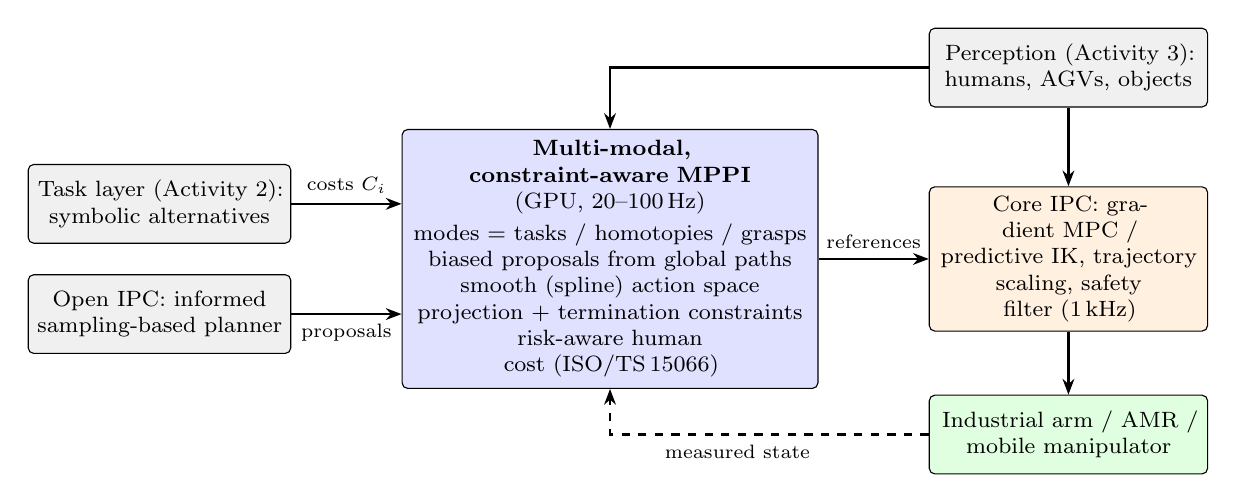
\begin{tikzpicture}[font=\footnotesize,
  blk/.style={draw,rounded corners=2pt,align=center,minimum height=10mm,fill=#1!12},
  arr/.style={-{Stealth[length=2mm]},thick}]
\node[blk=blue, text width=5.0cm, inner sep=4pt] (mppi) at (0,0) {\textbf{Multi-modal, constraint-aware MPPI}\\(GPU, 20--100\,Hz)\\[2pt]
  modes = tasks / homotopies / grasps\\ biased proposals from global paths\\ smooth (spline) action space\\ projection + termination constraints\\ risk-aware human cost (ISO/TS\,15066)};
\node[blk=gray, text width=3.1cm, anchor=east] (task) at ([xshift=-14mm,yshift=7mm]mppi.west) {Task layer (Activity 2):\\symbolic alternatives};
\node[blk=gray, text width=3.1cm, anchor=east] (glob) at ([xshift=-14mm,yshift=-7mm]mppi.west) {Open IPC: informed sampling-based planner};
\node[blk=orange, text width=3.3cm, anchor=west] (core) at ([xshift=14mm]mppi.east) {Core IPC: gradient MPC /\\predictive IK, trajectory\\scaling, safety filter (1\,kHz)};
\node[blk=gray, text width=3.3cm, anchor=south] (perc) at ([yshift=10mm]core.north) {Perception (Activity 3):\\humans, AGVs, objects};
\node[blk=green, text width=3.3cm, anchor=north] (rob) at ([yshift=-8mm]core.south) {Industrial arm / AMR /\\mobile manipulator};
\draw[arr] (task.east) -- node[above]{\scriptsize costs $C_i$} (task.east -| mppi.west);
\draw[arr] (glob.east) -- node[below]{\scriptsize proposals} (glob.east -| mppi.west);
\draw[arr] (mppi.east) -- node[above]{\scriptsize references} (core.west);
\draw[arr] (perc.west) -| (mppi.north);
\draw[arr] (perc.south) -- (core.north);
\draw[arr] (core.south) -- (rob.north);
\draw[arr,dashed] (rob.west) -| node[below,pos=0.3]{\scriptsize measured state} (mppi.south);
\end{tikzpicture}
\caption{Positioning of an MPPI-based local planner within the Plan4ARI architecture, as suggested by the gap analysis.}\label{fig:arch}
\end{figure}

These findings motivate the framework proposed for Plan4ARI (Fig.~\ref{fig:arch}): an MPPI layer that (a) samples task and homotopy alternatives in parallel as in M3P2I but keeps modes separated before the update, (b) draws part of its proposals from Open-IPC global paths and ancillary controllers, (c) enforces kinematic and separation constraints by projection and termination instead of penalties, and (d) hands smooth references to a gradient-based Core-IPC MPC that certifies joint, jerk and torque limits and scales the trajectory online~\cite{faroni2019pik,faroni2020scaling}. In this split MPPI provides reactivity and expressiveness, and classical MPC provides the guarantees that industrial deployment requires.

% ---------------------------------------------------------------------
\section{Conclusions}
% ---------------------------------------------------------------------
MPPI has matured into a credible basis for reactive motion planning: a sound stochastic-optimal-control foundation, open GPU implementations, adoption in the ROS\,2 navigation stack, and recent demonstrations on 7-DoF and dual-arm manipulators, contact-rich tasks and human-shared workspaces. Its main open issues for industrial robotics, namely constraint certification, mode averaging, sample efficiency in high dimensions and deterministic timing, are being addressed separately by distinct research lines. Combining them in a single multimodal, constraint-aware MPPI layer coupled with a certified gradient-based MPC is the direction proposed for Plan4ARI.

\fi
) omits Scope, Gap analysis and Conclusions
\newif\ifsotafull
\sotafulltrue


\title{\textbf{Model Predictive Path Integral Control for Industrial Manipulators and Autonomous Mobile Robots: a State-of-the-Art Analysis}\\[4pt]
\large Plan4ARI -- Activity 4, Task 4.1 -- Supporting note for D4.1 (A4 revision)}
\author{CNR-STIIMA, Industrial Robotics Lab}
\date{October 2026 -- Draft v0.1}

\begin{document}
\maketitle

\begin{abstract}
\noindent
Model Predictive Path Integral (MPPI) control is a sampling-based, derivative-free formulation of receding-horizon optimal control that maps naturally onto massively parallel hardware. In the last decade it has evolved from an aggressive-driving controller into a family of methods used for whole-body manipulation, contact-rich tasks, reactive task-and-motion planning and crowd-aware navigation, and it is now the reference predictive controller of the ROS\,2 navigation stack. This note reviews the theoretical foundations of MPPI, positions it with respect to gradient-based Model Predictive Control (MPC) and other horizon-based planners, and analyses the most promising contributions for industrial arms and AMRs, with a detailed discussion of the Multi-Modal MPPI of Zhang \emph{et al.}~\cite{zhang2024m3p2i}. We close with a gap analysis that motivates the MPPI-based motion-planning framework proposed for Plan4ARI.
\end{abstract}

% sota_body.tex -- body of the MPPI state-of-the-art note.
% Included by main.tex (standalone SOTA note) and by the D4.1 deliverable (D4.1-latex).
% Requires: amsmath, bm, algorithm, algpseudocode, tikz (arrows.meta, positioning), tabularx, booktabs, sota_macros.tex.
% ---------------------------------------------------------------------
\ifsotafull
\section{Scope and motivation}
% ---------------------------------------------------------------------
Plan4ARI targets teams of mobile manipulators and industrial arms working in dynamic, human-shared environments. Its baseline architecture couples informed sampling-based planning (global, \emph{Open IPC}) with MPC-based reference generation and micro-interpolation (local, \emph{Core IPC}). Two requirements stress this baseline: (i) \emph{reactivity}, i.e.\ replanning within tens of milliseconds when humans, AGVs or objects move, and (ii) \emph{expressiveness of the objective}: non-smooth costs (collision, separation distance, task switching, contact) that are awkward for gradient-based solvers. MPPI addresses both: it optimises an arbitrary cost by forward-simulating thousands of perturbed control sequences in parallel and averaging them with information-theoretic weights~\cite{williams2017jgcd,williams2018tro}. The review below was built from 69 sources (52 retrieved as full text and organised in an LLM-maintained wiki, see \texttt{../wiki/index.md}); recent surveys~\cite{kazim2024survey} were used to cross-check coverage.

\fi
% ---------------------------------------------------------------------
\section{Theoretical framework}
% ---------------------------------------------------------------------
\paragraph{Path integral control.}
Consider control-affine stochastic dynamics $d\bm{x} = \bm{f}(\bm{x})dt + \bm{G}(\bm{x})(\bm{u}\,dt + d\bm{w})$, $\E[d\bm{w}\,d\bm{w}^\top]=\bm{\Sigma}\,dt$, and the cost $J=\E\big[\phi(\bm{x}_T)+\int_0^T q(\bm{x}_t)+\tfrac12\bm{u}_t^\top\bm{R}\bm{u}_t\,dt\big]$. The value function obeys a nonlinear Hamilton--Jacobi--Bellman (HJB) PDE. Kappen~\cite{kappen2005pathintegrals} showed that, under the assumption $\lambda\bm{R}^{-1}=\bm{\Sigma}$ (noise is large where control is cheap), the exponential transformation $V=-\lambda\log\Psi$ makes the HJB \emph{linear} in the desirability $\Psi$. Through the Feynman--Kac lemma the solution becomes an expectation over uncontrolled trajectories,
\begin{equation}
\Psi(\bm{x}_0,0)=\E_{p}\!\left[\exp\!\big(-\tfrac{1}{\lambda}S(\tau)\big)\right],\qquad
\bm{u}^*(t)\,dt=\frac{\E_{p}\!\left[\exp(-S(\tau)/\lambda)\,d\bm{w}_t\right]}{\E_{p}\!\left[\exp(-S(\tau)/\lambda)\right]},
\label{eq:pi}
\end{equation}
where $S(\tau)=\phi(\bm{x}_T)+\int q\,dt$ is the state cost of trajectory $\tau$. The optimal control is thus a \emph{cost-weighted average of noise}, computable by Monte-Carlo sampling without differentiating dynamics or cost. Theodorou \emph{et al.}~\cite{theodorou2010pi2} exploited this result for policy improvement (PI$^2$), and STOMP~\cite{kalakrishnan2011stomp} for offline trajectory optimisation.

\paragraph{Information-theoretic MPPI.}
Williams \emph{et al.} turned \eqref{eq:pi} into a receding-horizon controller~\cite{williams2016aggressive,williams2017jgcd} and later re-derived it in discrete time from an information-theoretic argument that removes the control-affine assumption~\cite{williams2017itmpc,williams2018tro}. Let $\V=(\bm{v}_0,\dots,\bm{v}_{T-1})$ be an input sequence sampled as $\bm{v}_t=\bm{u}_t+\bm{\epsilon}_t$, $\bm{\epsilon}_t\sim\mathcal{N}(\bm 0,\bm\Sigma)$, with density $q_{\U}$, and let $p$ be a base (prior) distribution. The free energy satisfies
\begin{equation}
-\lambda\log\E_{p}\!\left[e^{-S(\V)/\lambda}\right]\;\le\;\E_{q}[S(\V)]+\lambda\,\KL(q\,\|\,p),
\end{equation}
with equality for the optimal distribution $q^*(\V)=\eta^{-1}\exp(-S(\V)/\lambda)\,p(\V)$. MPPI chooses the Gaussian mean $\U$ that minimises $\KL(q^*\|q_{\U})$, which yields a closed-form importance-sampling estimate from $K$ rollouts:
\begin{equation}
\bm{u}_t\leftarrow\bm{u}_t+\sum_{k=1}^{K}w_k\,\bm{\epsilon}^k_t,\qquad
w_k=\frac{1}{\eta}\exp\!\Big(-\frac{1}{\lambda}\big(\tilde S_k-\rho\big)\Big),\qquad
\tilde S_k=S(\V_k)+\gamma\sum_{t}\bm{u}_t^\top\bm\Sigma^{-1}\bm{v}^k_t,
\label{eq:mppi}
\end{equation}
where $\rho=\min_k\tilde S_k$ ensures numerical stability, $\eta$ normalises the weights, and the second term of $\tilde S_k$ is the likelihood-ratio (control) cost arising from the change of measure ($\gamma=\lambda(1-\alpha)$ in~\cite{williams2018tro}). The \emph{inverse temperature} $1/\lambda$ interpolates between a plain average ($\lambda\to\infty$) and greedy selection of the best rollout ($\lambda\to0$). Algorithm~\ref{alg:mppi} summarises one control cycle; the warm-started, shifted mean makes MPPI an anytime, real-time-iteration scheme.

\begin{algorithm}[t]
\caption{One cycle of MPPI (receding horizon)}\label{alg:mppi}
\begin{algorithmic}[1]
\small
\Require state $\bm{x}_0$, nominal sequence $\U$, covariance $\bm\Sigma$, temperature $\lambda$, samples $K$, horizon $T$
\For{$k=1\dots K$ \textbf{in parallel}}
  \State sample $\bm{\epsilon}^k_{0:T-1}\sim\mathcal{N}(\bm 0,\bm\Sigma)$; \quad roll out $\bm{x}^k_{t+1}=\bm{F}(\bm{x}^k_t,\bm{u}_t+\bm{\epsilon}^k_t)$ \Comment{model or physics simulator}
  \State $\tilde S_k\gets \phi(\bm{x}^k_T)+\sum_t q(\bm{x}^k_t)+\gamma\,\bm{u}_t^\top\bm\Sigma^{-1}(\bm{u}_t+\bm{\epsilon}^k_t)$
\EndFor
\State $\rho\gets\min_k\tilde S_k$;\quad $w_k\gets\exp(-(\tilde S_k-\rho)/\lambda)/\eta$ \Comment{importance weights}
\State $\bm{u}_t\gets\bm{u}_t+\sum_k w_k\bm{\epsilon}^k_t$; optionally smooth $\U$ \Comment{e.g.\ Savitzky--Golay, splines}
\State apply $\bm{u}_0$; shift $\U$ by one step and re-initialise $\bm{u}_{T-1}$ \Comment{warm start}
\end{algorithmic}
\end{algorithm}

\paragraph{Properties and limitations.}
MPPI (i) needs neither gradients nor convexity, so collision indicators, costmaps, logical task predicates and contacts enter the cost directly; (ii) is embarrassingly parallel (GPU, and recently FPGA~\cite{desai2026fpgampi}); (iii) can use a black-box physics engine as model~\cite{pezzato2025isaacmppi,howell2022predictivesampling}. Its known weaknesses are equally relevant for industrial use: constraints are only soft (penalties), so feasibility is not certified; sample complexity grows with input dimension and horizon; the Gaussian proposal is unimodal and the weighted \emph{average} of rollouts belonging to different homotopy classes can be infeasible (``averaging-induced failure''~\cite{liu2026clusteringmppi}); injected noise produces chattering inputs~\cite{kim2022smppi}; and stability or recursive-feasibility guarantees of classical MPC~\cite{mayne2014mpc} do not carry over. Most of the literature reviewed in Sect.~\ref{sec:lit} addresses one of these points.

% ---------------------------------------------------------------------
\section{MPPI versus MPC and other horizon-based planners}\label{sec:cmp}
% ---------------------------------------------------------------------
Gradient-based nonlinear MPC (NMPC) solves at each step a deterministic nonlinear program, typically with SQP or interior-point methods and real-time iterations (e.g.\ \texttt{acados}~\cite{verschueren2022acados}); it handles hard state/input constraints, provides local optimality and, with terminal ingredients, stability and recursive feasibility~\cite{rawlings2017mpc,mayne2014mpc}. It is the natural tool for jerk/torque-limited reference generation, as in predictive inverse kinematics and trajectory scaling for industrial manipulators~\cite{faroni2019pik,faroni2020scaling}. Its weaknesses are the need for smooth models and costs, sensitivity to initialisation in non-convex scenes (it converges to the local minimum of the current homotopy class), and the difficulty of encoding contacts and discrete decisions. Differential dynamic programming/iLQR~\cite{tassa2012ilqg} shares these traits but adds time-varying feedback gains.

Sampling-based MPC replaces the NLP with a stochastic search. The Cross-Entropy Method~\cite{rubinstein1999cem,pinneri2020icem} refits a Gaussian on an elite subset, predictive sampling~\cite{howell2022predictivesampling} keeps the best sample, and MPPI uses soft Boltzmann weights; Wagener \emph{et al.}~\cite{wagener2019dmd} unified these schemes as instances of online (mirror-descent) learning, and Stein-variational MPC~\cite{lambert2020svmpc} generalises them to non-parametric, multimodal posteriors. Classical motion-planning trajectory optimisers (CHOMP, STOMP, TrajOpt~\cite{zucker2013chomp,kalakrishnan2011stomp,schulman2014trajopt}) solve similar problems offline over full paths, while mobile-robot local planners such as DWA~\cite{fox1997dwa} (one-step constant-velocity sampling) and TEB~\cite{rosmann2017teb} (sparse NLP over multiple topologies) are the industrial incumbents MPPI is replacing in Nav2~\cite{macenski2023nav2survey}. Table~\ref{tab:cmp} summarises the comparison.

\begin{table}[t]
\centering\small
\caption{Qualitative comparison of horizon-based planning/control methods relevant to Plan4ARI.}\label{tab:cmp}
\setlength{\tabcolsep}{4pt}
\begin{tabularx}{\textwidth}{@{}>{\raggedright}p{2.3cm}>{\raggedright}X>{\raggedright}X>{\raggedright}X>{\raggedright}X>{\raggedright\arraybackslash}X@{}}
\toprule
 & \textbf{NMPC (SQP/IPM)} & \textbf{iLQR / DDP} & \textbf{CEM / predictive sampling} & \textbf{MPPI and variants} & \textbf{DWA / TEB} \\
\midrule
Optimisation principle & Deterministic NLP, Newton-type & Riccati backward pass & Elite refit / best sample & Path-integral importance sampling & Velocity sampling / sparse NLP \\
Gradients of model \& cost & Required (2nd order) & Required & Not required & Not required & DWA: no; TEB: yes \\
Hard constraints & Yes (exact) & Via augmented Lagrangian & Penalties / rejection & Penalties; CBF, projection or termination in variants & Partially \\
Non-smooth cost, contacts, logic & Poor & Poor & Good & Good (simulator in the loop) & Limited \\
Multimodality & Single local optimum & Single local optimum & Unimodal Gaussian & Unimodal; multimodal in SVMPC, SVG-, M3P2I, CE-MPPI & TEB: parallel topologies \\
Theory & Stability, recursive feasibility & Local convergence & Weak & Free-energy optimality; tube/robust bounds~\cite{gandhi2021rmppi} & Heuristic \\
Typical rate (arm / AMR) & 100--1000\,Hz (small models) & 100--1000\,Hz & 20--200\,Hz on GPU & 20--170\,Hz on GPU & 10--50\,Hz \\
Industrial maturity & High (\texttt{acados}, PLC-grade) & Medium & Research & ROS\,2 Nav2, STORM, MPPI-Generic & High (ROS) \\
\bottomrule
\end{tabularx}
\end{table}

The emerging consensus is that the two families are complementary rather than competing: MPPI explores globally within the horizon and copes with non-smooth objectives, gradient-based MPC refines and certifies. Hybrid schemes already appear at both levels: cuRobo~\cite{sundaralingam2023curobo} seeds GPU L-BFGS with a particle-based (MPPI-like) optimiser and plans collision-free arm motions in about 30--50\,ms, while Aoyama \emph{et al.}~\cite{aoyama2026hybrid} alternate DDP steps with Hessian-shaped sampling to escape local minima.

% ---------------------------------------------------------------------
\section{Analysis of the literature}\label{sec:lit}
% ---------------------------------------------------------------------
\subsection{Algorithmic advances}
\paragraph{Robustness to disturbances and model error.} Tube-MPPI~\cite{williams2018tubemppi} pairs MPPI with an iLQG ancillary tracker; RMPPI~\cite{gandhi2021rmppi} adds an augmented nominal state and provides bounds on the free-energy growth, i.e.\ the first performance guarantee for MPPI. Ensemble MPPI~\cite{abraham2020emppi} samples model parameters and adapts them online; U-MPPI~\cite{mohamed2025umppi} propagates means and covariances with the unscented transform and adds risk-sensitive costs; covariance steering~\cite{yin2022covsteering} shapes the sampled trajectory distribution.

\paragraph{Constraints and safety.} This is the most active line and the most relevant for certification. Shield-MPPI~\cite{yin2023shieldmppi} and SC-MPPI~\cite{gandhi2023safeis} embed control barrier functions (CBFs) in the cost or directly in forward sampling; GS-MPPI~\cite{rabiee2025gsmppi} uses composite CBFs so that \emph{all} sampled trajectories are safe; BR-MPPI~\cite{parwana2025brmppi} treats barrier rates as additional inputs and projects samples on the constraint manifold; BSS-MPPI~\cite{yin2024ccmppi} enforces chance constraints in belief space. For manipulators, PR-MPPI~\cite{lee2026prmppi} projects sampled joint velocities on equality (closed-chain) and inequality (joint-limit, clearance) constraints and retracts the result, achieving exact constraint satisfaction on 14-DoF dual-arm systems, while COSMIK-MPPI~\cite{gursoy2026cosmik} enforces human--robot separation by treating violations as rollout terminations (\emph{constraints-as-terminations}) and reports 100\% success at a constant 22\,ms per cycle, where gradient-based MPC failed in cluttered scenes.

\paragraph{Sampling distribution, smoothness and multimodality.} Smooth-MPPI~\cite{kim2022smppi} samples in the derivative-action space to remove chattering without post-filtering; log-MPPI~\cite{mohamed2022logmppi} uses normal--log-normal noise for better exploration of costmaps; Biased-MPPI~\cite{trevisan2024biasedmppi} re-derives MPPI for arbitrary proposal distributions and mixes samples from ancillary controllers (e.g.\ a global planner, a learned policy, a braking controller), alleviating local minima. MPOPI~\cite{asmar2023mpopi} adapts the proposal through adaptive importance sampling, and Tsallis-divergence VI-MPC~\cite{wang2021tsallis} generalises the exponential weighting. Multimodality is handled by Stein variational methods (SVMPC~\cite{lambert2020svmpc}, SVG-MPPI~\cite{honda2024svgmppi}), by clustering rollouts into homotopy modes before averaging (CE-MPPI~\cite{liu2026clusteringmppi}, 48\% shorter time-to-goal on a UR5e), and by learned proposals~\cite{sacks2023learningsampling}. Diffusion-style annealing~\cite{xue2025dialmpc,pan2024mbd} is a recent reinterpretation of the iterated path-integral update as score-based denoising.

\paragraph{Learning-augmented MPPI.} MPPI is the planner of several model-based RL agents (POLO, MPQ, TD-MPC~\cite{lowrey2019polo,bhardwaj2020mpq,hansen2022tdmpc}) where a learned terminal value extends the effective horizon, a relevant feature for long industrial tasks with short real-time horizons.

\subsection{Industrial and collaborative manipulators}
STORM~\cite{bhardwaj2021storm} is the reference joint-space MPPI for 7-DoF arms: GPU rollouts of the kinematic chain, learned self-collision and signed-distance costs, Halton-spline sampling, and a 125\,Hz control rate with task- and joint-space constraints as costs. Pezzato \emph{et al.}~\cite{pezzato2025isaacmppi} replace the hand-coded model with Isaac\,Gym~\cite{makoviychuk2021isaacgym}, solving navigation, non-prehensile pushing and whole-body mobile manipulation with 750 parallel simulations at 25\,Hz, thus removing the need for explicit contact models. Contact-rich deployment with MuJoCo-MJX/JAX on a Franka arm~\cite{dierking2026parallelsbmpc} shows that structured multimodal sampling outperforms unimodal CEM/MPPI, but also that fidelity of contact modelling and the compute budget (8--10\,Hz planning) remain bottlenecks. At the torque level, Im \emph{et al.}~\cite{im2026torquemppi} sample joint torques through full rigid-body dynamics, obtaining compliant, force-aware behaviour at 166\,Hz with a 0.18\,s horizon on a 7-DoF arm. VP-STO~\cite{jankowski2023vpsto} applies the same stochastic philosophy to via-point parametrised, time-optimal trajectories, an attractive representation for industrial controllers that expect smooth, bounded references. For HRC, COSMIK-MPPI~\cite{gursoy2026cosmik} closes the loop with markerless human pose estimation, which is directly aligned with the ISO/TS~15066 speed-and-separation monitoring paradigm.

\subsection{Mobile robots and AMRs}
MPPI was born on the AutoRally platform for aggressive driving~\cite{williams2016aggressive,williams2018tro}. For indoor AMRs the key milestone is its adoption in ROS\,2 Nav2, where the maintainers report that it rarely needs recovery behaviours and plan to make it the default local controller~\cite{macenski2023nav2survey}. Mohamed \emph{et al.} address navigation in unknown cluttered spaces with log-MPPI~\cite{mohamed2022logmppi}, Gaussian-process subgoal guidance (GP-MPPI~\cite{mohamed2023gpmppi}) and unscented sampling~\cite{mohamed2025umppi}. Human-aware navigation is the second major theme: DRA-MPPI~\cite{trevisan2025drampi} evaluates Monte-Carlo collision probabilities against non-Gaussian pedestrian predictions for hundreds of rollouts in real time, mitigating the freezing-robot problem; interaction-aware~\cite{jansma2023interaction} and multi-agent path-integral formulations~\cite{streichenberg2023mapi} couple the plans of several agents, a building block for fleets of AMRs. Contingency-MPPI~\cite{jung2024contingency} guarantees that a safe fallback plan always exists, and the FPGA design of~\cite{desai2026fpgampi} reduces latency (3.1--7.5$\times$) and energy (2.5--5.4$\times$) on battery-powered embedded platforms.

\subsection{In-depth: Multi-Modal MPPI and Active Inference for reactive TAMP}
Zhang \emph{et al.}~\cite{zhang2024m3p2i} address \emph{reactive} task-and-motion planning, the closest problem to Plan4ARI's mobile-manipulation scenarios. A high-level Active Inference planner (AIP)~\cite{pezzato2023aip}, guided by a Behaviour Tree, reasons on symbolic beliefs and is modified to return not one but $N$ \emph{alternative} plans (e.g.\ \texttt{push} vs.\ \texttt{pull}, top vs.\ side grasp); each first action is linked through a plan interface to a cost function $C_i$. The low-level Multi-Modal MPPI (M3P2I) then samples $N\!\cdot\!K$ control sequences in Isaac\,Gym, $K$ per alternative, with Halton-spline noise. Weights are first computed \emph{per alternative}, $\omega_i(\V_k)\propto\exp(-(S_i(\V_k)-\rho_i)/\beta_i)$, with the inverse temperature $\beta_i$ auto-tuned so that the effective sample count $\eta_i$ stays in 5--10\% of $K$; the per-mode means $\mu_i$ are then concatenated and re-weighted jointly to produce a single command $u_t=(1-\alpha_u)u_{t-1}+\alpha_u\sum_k\tilde\omega_k v_{t,k}$. The action planner runs at about 1\,Hz and M3P2I at 25\,Hz.

\emph{Results.} In a push--pull task with an omnidirectional base, the multimodal controller always succeeded, whereas push-only timed out when the object lay in a corner; mean orientation error dropped from 0.0198 (push) and 0.0777 (pull) to 0.0041 and execution time from 6.2--25.1\,s to 3.8\,s (object in the middle). In a 7-DoF pick-and-place task with disturbances (moved/stolen cube, dynamic obstacles) it outperformed an Isaac\,Gym actor-critic RL baseline (position error 0.0117 vs.\ 0.0246\,m) without any training, and it blended top and side grasps according to the geometry; real experiments on a Franka Panda confirmed recovery from disturbances.

\emph{Assessment for Plan4ARI.} The key idea, moving the choice between discrete alternatives from hand-written task-level heuristics to parallel sampling at the motion level, is directly reusable for alternative grasps, approach directions, base placements or homotopy classes produced by a global planner. Its limitations are equally instructive: (i) the final weighted blending can still average incompatible modes (the issue later formalised by CE-MPPI~\cite{liu2026clusteringmppi}); (ii) all constraints, including obstacle avoidance, are soft costs with manually tuned weights; (iii) computation scales with $N\!\cdot\!K$ full physics rollouts, and fidelity depends on the simulator (sim-to-real handled only by randomisation); (iv) no explicit treatment of humans or safety standards. These gaps are complementary to those solved by the constraint-aware and risk-aware variants above.

\subsection{Software ecosystem}
Mature open-source implementations exist: MPPI-Generic (CUDA, C++)~\cite{vlahov2024mppigeneric}, the Nav2 MPPI controller~\cite{macenski2023nav2survey}, STORM and cuRobo for arms~\cite{bhardwaj2021storm,sundaralingam2023curobo}, Isaac\,Gym-based MPPI~\cite{pezzato2025isaacmppi}, MuJoCo predictive sampling~\cite{howell2022predictivesampling} and JAX/MJX pipelines~\cite{dierking2026parallelsbmpc}. None of them, however, targets the deterministic timing and safety-rated interfaces of industrial controllers.

\ifsotafull
% ---------------------------------------------------------------------
\section{Gap analysis and implications for the proposed framework}\label{sec:gap}
% ---------------------------------------------------------------------
The review exposes five gaps relevant to Plan4ARI:
\begin{enumerate}
\item \textbf{Certified constraint satisfaction.} Penalty-based MPPI cannot guarantee joint, jerk, torque or separation-distance limits; projection/termination/CBF variants~\cite{lee2026prmppi,gursoy2026cosmik,rabiee2025gsmppi} are promising but have not been combined with industrial reference interfaces.
\item \textbf{Multimodality across task and motion.} M3P2I~\cite{zhang2024m3p2i} and CE-MPPI~\cite{liu2026clusteringmppi} show the value of sampling alternatives in parallel, but no method selects among modes \emph{and} preserves a single feasible mode in the command.
\item \textbf{Unified arm/AMR (whole-body) planning} in human-shared spaces is shown only in simulation-heavy demonstrations~\cite{pezzato2025isaacmppi}; human-risk models~\cite{trevisan2025drampi} exist for AMRs but not for mobile manipulators.
\item \textbf{Global--local coupling.} Biased-MPPI~\cite{trevisan2024biasedmppi} allows global planners to act as proposal distributions, a natural bridge to the informed sampling-based planners of the Open IPC that has not yet been exploited with multi-path reuse.
\item \textbf{Real-time determinism.} GPU-based MPPI typically runs at 20--170\,Hz; industrial axes require 1\,kHz smooth, bounded references, so a certified downstream layer remains necessary.
\end{enumerate}

\begin{figure}[t]
\centering
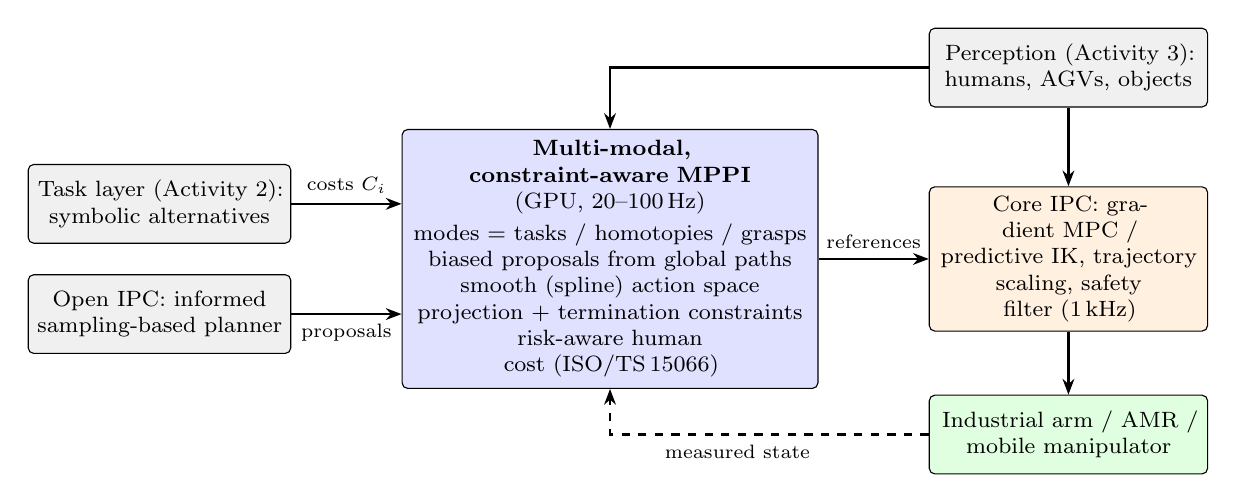
\begin{tikzpicture}[font=\footnotesize,
  blk/.style={draw,rounded corners=2pt,align=center,minimum height=10mm,fill=#1!12},
  arr/.style={-{Stealth[length=2mm]},thick}]
\node[blk=blue, text width=5.0cm, inner sep=4pt] (mppi) at (0,0) {\textbf{Multi-modal, constraint-aware MPPI}\\(GPU, 20--100\,Hz)\\[2pt]
  modes = tasks / homotopies / grasps\\ biased proposals from global paths\\ smooth (spline) action space\\ projection + termination constraints\\ risk-aware human cost (ISO/TS\,15066)};
\node[blk=gray, text width=3.1cm, anchor=east] (task) at ([xshift=-14mm,yshift=7mm]mppi.west) {Task layer (Activity 2):\\symbolic alternatives};
\node[blk=gray, text width=3.1cm, anchor=east] (glob) at ([xshift=-14mm,yshift=-7mm]mppi.west) {Open IPC: informed sampling-based planner};
\node[blk=orange, text width=3.3cm, anchor=west] (core) at ([xshift=14mm]mppi.east) {Core IPC: gradient MPC /\\predictive IK, trajectory\\scaling, safety filter (1\,kHz)};
\node[blk=gray, text width=3.3cm, anchor=south] (perc) at ([yshift=10mm]core.north) {Perception (Activity 3):\\humans, AGVs, objects};
\node[blk=green, text width=3.3cm, anchor=north] (rob) at ([yshift=-8mm]core.south) {Industrial arm / AMR /\\mobile manipulator};
\draw[arr] (task.east) -- node[above]{\scriptsize costs $C_i$} (task.east -| mppi.west);
\draw[arr] (glob.east) -- node[below]{\scriptsize proposals} (glob.east -| mppi.west);
\draw[arr] (mppi.east) -- node[above]{\scriptsize references} (core.west);
\draw[arr] (perc.west) -| (mppi.north);
\draw[arr] (perc.south) -- (core.north);
\draw[arr] (core.south) -- (rob.north);
\draw[arr,dashed] (rob.west) -| node[below,pos=0.3]{\scriptsize measured state} (mppi.south);
\end{tikzpicture}
\caption{Positioning of an MPPI-based local planner within the Plan4ARI architecture, as suggested by the gap analysis.}\label{fig:arch}
\end{figure}

These findings motivate the framework proposed for Plan4ARI (Fig.~\ref{fig:arch}): an MPPI layer that (a) samples task and homotopy alternatives in parallel as in M3P2I but keeps modes separated before the update, (b) draws part of its proposals from Open-IPC global paths and ancillary controllers, (c) enforces kinematic and separation constraints by projection and termination instead of penalties, and (d) hands smooth references to a gradient-based Core-IPC MPC that certifies joint, jerk and torque limits and scales the trajectory online~\cite{faroni2019pik,faroni2020scaling}. In this split MPPI provides reactivity and expressiveness, and classical MPC provides the guarantees that industrial deployment requires.

% ---------------------------------------------------------------------
\section{Conclusions}
% ---------------------------------------------------------------------
MPPI has matured into a credible basis for reactive motion planning: a sound stochastic-optimal-control foundation, open GPU implementations, adoption in the ROS\,2 navigation stack, and recent demonstrations on 7-DoF and dual-arm manipulators, contact-rich tasks and human-shared workspaces. Its main open issues for industrial robotics, namely constraint certification, mode averaging, sample efficiency in high dimensions and deterministic timing, are being addressed separately by distinct research lines. Combining them in a single multimodal, constraint-aware MPPI layer coupled with a certified gradient-based MPC is the direction proposed for Plan4ARI.

\fi


\bibliographystyle{IEEEtran}
\bibliography{references}

\end{document}
